\documentclass[12pt, letterpaper, titlepage]{article}

\usepackage{amsmath}
\usepackage{booktabs}
\usepackage{amsthm}
\usepackage{graphicx}
\usepackage[margin=1in]{geometry}
\usepackage{hyperref}
\hypersetup{colorlinks = true, linkcolor = blue, citecolor=blue, urlcolor = blue}
\usepackage{natbib}
\usepackage{enumitem}
\usepackage{setspace}

\usepackage[pagewise]{lineno}
%\linenumbers*[1]
% %% patches to make lineno work better with amsmath
\newcommand*\patchAmsMathEnvironmentForLineno[1]{%
 \expandafter\let\csname old#1\expandafter\endcsname\csname #1\endcsname
 \expandafter\let\csname oldend#1\expandafter\endcsname\csname end#1\endcsname
 \renewenvironment{#1}%
 {\linenomath\csname old#1\endcsname}%
 {\csname oldend#1\endcsname\endlinenomath}}%
\newcommand*\patchBothAmsMathEnvironmentsForLineno[1]{%
 \patchAmsMathEnvironmentForLineno{#1}%
 \patchAmsMathEnvironmentForLineno{#1*}}%

\AtBeginDocument{%
 \patchBothAmsMathEnvironmentsForLineno{equation}%
 \patchBothAmsMathEnvironmentsForLineno{align}%
 \patchBothAmsMathEnvironmentsForLineno{flalign}%
 \patchBothAmsMathEnvironmentsForLineno{alignat}%
 \patchBothAmsMathEnvironmentsForLineno{gather}%
 \patchBothAmsMathEnvironmentsForLineno{multline}%
}

% control floats
\renewcommand\floatpagefraction{.9}
\renewcommand\topfraction{.9}
\renewcommand\bottomfraction{.9}
\renewcommand\textfraction{.1}
\setcounter{totalnumber}{50}
\setcounter{topnumber}{50}
\setcounter{bottomnumber}{50}

\newcommand{\jy}[1]{\textcolor{blue}{JY: #1}}
\newcommand{\eds}[1]{\textcolor{red}{EDS: (#1)}}


\title{Time Series Length at Which Block Bootstrapping is Effective for Estimation of Variance}

\author{Mathew Chandy\\
%   \href{mailto:mathew.chandy@uconn.edu}
% {\nolinkurl{mathew.chandy@uconn.edu}}\\
  Jun Yan\\[1ex]
  Department of Statistics, University of Connecticut\\
}
\date{}

\begin{document}
\maketitle

\doublespace

\begin{abstract}
Block bootstrapping is a method that can be used for estimating a statistic of a time
series. It involves splitting a series into blocks (in order to account for the time
factor) and re-sampling the blocks to create many new bootstrapped time series.
This method becomes more effective as the length of the time series increases. 
The question for this study is how does one determine at what length the block
bootstrap method stops being an effective method to estimate a statistic of a time
series.

\bigskip
\noindent\sc{Keywords}:
block bootstrap;
\end{abstract}

\section{Introduction}
\label{sec:intro}

For this study, many block bootstrap simulations were conducted with R. At the base
level, we are block-bootstrapping an auto-regressive process with true mean 0.
Bootstrapping is the term for creating new samples of the same size by re-sampling from
the original sample with replacement. Many bootstrapped samples are used to create a
distribution of sampling means to estimate mean and variance. This works for samples
that are not dependent. However, for a time series such as an auto-regressive process,
a different procedure is required to account for the time dependence. In such a case,
the series is split into blocks that may overlap (moving block bootstrap) or may not
overlap (non-moving block bootstrap). These blocks are then re-sampled to create new
bootstrapped time series. 

In our experiment, we find the means of a 1000 block-bootstrapped time series, 
and create a 95 \% confidence interval of the means. We replicate this 1000 times, 
and record the proportion of confidence intervals that recover the true mean 
(coverage rate). We are effectively observing how successful the bootstrapping process
is at estimating the mean and variance. The key variable being observed was n, 
the length of the time series, or the size of the sample. It is known that as n
increases, block bootstrapping will become a less accurate method for estimation
(the coverage rates will decrease). The question is at what range of n values does this
start to become a problem. 

In this experiment, there are certain factors that are expected to affect the coverage
rates. As the Auto-Regressive (AR) coefficient (the time dependence) of the time series increases,
we expect the coverage rates of the confidence intervals to decrease.
The coverage rates are also affected by the size of the blocks - more specifically,
how the size of the blocks (l) relates to the size of the time series (n) - 
and whether or not they overlap.

So to solve the question of what n is necessary for effective block bootstrapping,
while still accounting for all these factors, the simulations were repeated for
multiple combinations of AR coefficient and the function of n used to decide l. In addition, the coverage rates
for both the non-moving and moving methods were recorded.

\section{Literature Review}
\label{sec:litreview}




\section{Data}
\label{sec:data}




\section{Methods}
\label{sec:methods}

A simulation of an autoregressive integrated moving average (ARIMA) process was run repeatedly with varying parameters. 
The mean and standard deviation of the time series was held constant at 0 and 0.1, whereas the sample size and AR Coefficient
 were varied. The AR Coefficients that were used were 0.2, 0.4, and 0.6. The sample sizes that were used depended on the AR
 Coefficient, and the function used to compute l. For each of these variations, 1000 confidence intervals are created using
 the block bootstrap method, and the proportion of these intervals that recover the true mean (0) is recorded as the coverage
 rate. The block bootstrap method has different settings that were varied in this study: non-moving vs moving, 
and the function for block length - the two used were a constant block length of 10 and the square root of n.

For the simulations using a constant block length of 10, the sample size was gradually lowered by increments of 20 to see when
the block bootstrap would begin to consistently return low coverage rates. For AR = 0.2 using a constant l, results for
sample sizes ranging from 400 to 20 were observed. For AR = 0.4 using a constant l, results for sample sizes ranging from 600
to 20 were observed. For AR = 0.6, using a constant l, results for sample sizes ranging from 900 to 220 were observed. For the simulations in which the block length was the square root of the time series length, the only sample sizes used were perfect squares so that the blocks would have whole number lengths. For AR = 0.2 using l = sqrt{n}, results for sample sizes ranging from 625 to 36 were observed. For AR = 0.4 using sqrt{n}, results for sample sizes ranging from 900 to 121 were observed. For AR = 0.6 using l = sqrt{n}, results for sample sizes ranging from 1600 to 121 were observed. 

\section{Results}

As the AR Coefficient increases, it was found unsurprisingly that a larger sample size was required for effective block bootstrap estimation. With l = sqrt{n} and AR = 0.2, all observed coverage rates are lower than .92 for n <= 225. For all n's <= 100, all observed coverage rates were below .90. With l = sqrt{n} and AR = 0.4, all observed coverage rates were below .92 for n <= 441. For all n's <= 144, all observed coverage rates were below .90. With l = sqrt{n} and AR = 0.6, all observed coverage rates were below .92 for n <= 400. For all n's <= 196, all observed coverage rates were below .90. 

With a constant l and AR = 0.2, for n <= 180, all observed coverage rates were below .92. For all n's <= 60, all observed coverage rates were below .90. With a constant l and AR = 0.4, for n <= 160, all observed coverage rates were below .91. For all n's <= 80, all observed coverage rates were below .90. With a constant l and AR = 0.6, for n <= 380, all observed coverage rates were below .92. For all n's <= 240, all observed coverage rates were below .90.



\begin{figure}[]
  \centering
  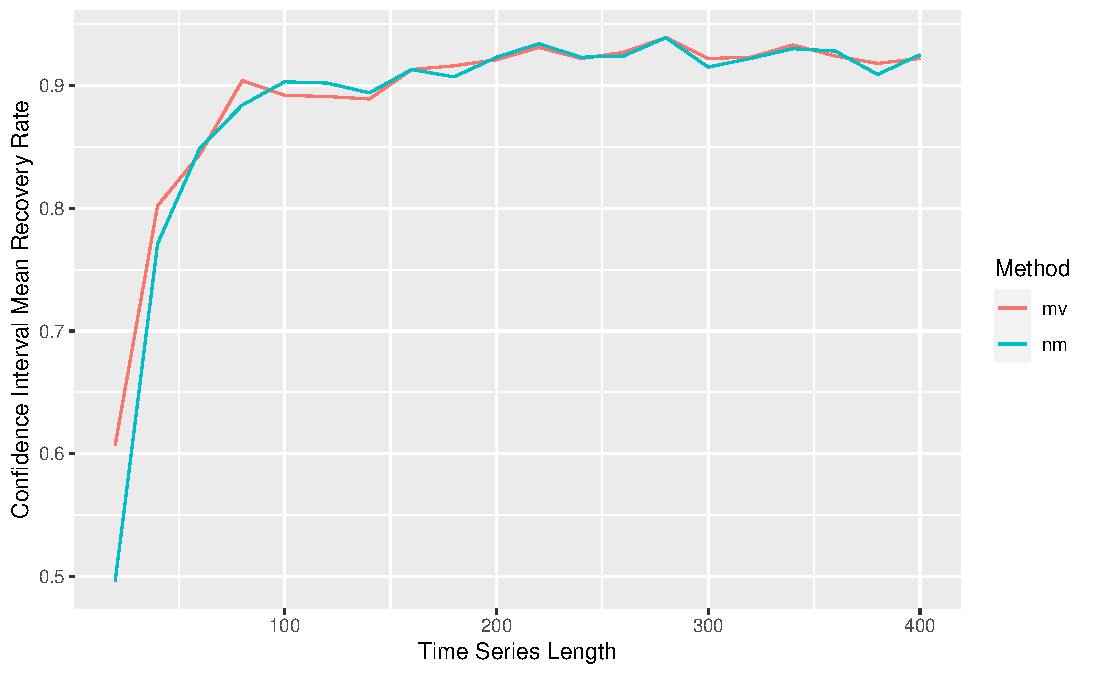
\includegraphics[width=\textwidth]{constant_0.2}
  \caption{}
  \label{fig:constant_0.2}
\end{figure}

\label{sec:results}




\section{Discussion}
\label{sec:discuss}



\bibliographystyle{chicago}
\bibliography{citations.bib}


\end{document}